\documentclass[11pt]{jsarticle}

\usepackage{amsmath,amsthm,amssymb}
\usepackage[dvipdfmx]{graphicx}
\usepackage{bm}
%
\usepackage{multirow}
\usepackage{wrapfig}
%
\pagestyle{empty}
%% 高さの設定
\setlength{\textheight}{\paperheight}   % ひとまず紙面を本文領域に
\setlength{\topmargin}{-5.4truemm}      % 上の余白を20mm(=1inch-5.4mm)に
\addtolength{\topmargin}{-\headheight}  % 
\addtolength{\topmargin}{-\headsep}     % ヘッダの分だけ本文領域を移動させる
\addtolength{\textheight}{-40truemm}    % 下の余白も20mmに%% 幅の設定
\setlength{\textwidth}{\paperwidth}     % ひとまず紙面を本文領域に
\setlength{\oddsidemargin}{-5.4truemm}  % 左の余白を20mm(=1inch-5.4mm)に
\setlength{\evensidemargin}{-5.4truemm} % 
\addtolength{\textwidth}{-40truemm}     % 右の余白も20mmに

%
\abovecaptionskip=-1pt
%\belowcaptionskip=-1pt
%
\renewcommand{\baselinestretch}{0.9} % 全体の行間調整
\renewcommand{\figurename}{Fig.}
\renewcommand{\tablename}{Tab.}
%
\makeatletter 
\def\section{\@startsection {section}{1}{\z@}{1.5 ex plus 2ex minus -.2ex}{0.5 ex plus .2ex}{\large\bf}}
\def\subsection{\@startsection{subsection}{2}{\z@}{0.2\Cvs \@plus.5\Cdp \@minus.2\Cdp}{0.1\Cvs \@plus.3\Cdp}{\reset@font\normalsize\bfseries}}
\makeatother 
%

\begin{document}

%%%%%%
% はじめに
%%%%%%
\begin{center}
{\Large \textgt{34. DPD シミュレーションによる動的ネットワークの緩和挙動の検討}}
\end{center}

\begin{flushright}
東亞合成 ${}^\circ$佐々木裕\\
近大理工 荒井規允

Tel: 052-611-9923, e-mail: hiroshi\_sasaki$@$mail.toagosei.co.jp
\end{flushright}

\vspace{0.5\baselineskip}
\section{はじめに}

近年、ソフトマター研究~\cite{DeGennes1992}の深化に伴い、ソフトマターの特徴である柔らかさに各種の新規機能を付加した材料の開発が活発に行われている。
力学的な機能を検討する場合には、系全体の流動を抑制した固体的な特性が要求され、ネットワーク構造が必要となる場合が多い。
構造の明確なネットワークの形成方法の一つとして、水素結合、疎水性相互作用、静電相互作用などの、共有結合よりも乖離障壁の低い「繋ぎ替え可能な非共有結合」を介して自己組織化した超分子ネットワークが報告されている~\cite{CHINO2005}。

超分子ネットワークの特徴的な構造をモデル化することを考えよう。
相互作用する化学種をセグメントとして粗視化し、それらのセグメント間に適正な相互作用パラメタ(引力あるいは斥力を表現)を設定することで、偏析したクラスタを介したネットワークモデルを得ることができる。
このようなモデルとして、もっとも簡単なものが、ポリマー鎖の両末端に偏析するセグメントを配したテレケリックポリマーである。

我々は、粗視化した超分子ネットワークのモデルとしてテレケリックポリマーを採用し、動的なネットワークの緩和挙動に注目して検討を行った。
ここでは、マクロに測定可能な応力緩和関数 $G(t)$ から算出した緩和時間と、ミクロな構造に起因した緩和時間である、末端間ベクトルの自己相関、および、末端ビーズが偏析したドメインからの引き抜きから算出した緩和時間とを比較した結果について報告を行う。

\section{シミュレーション}

本研究では散逸粒子動力学(DPD)法~\cite{Groot1997}を使用した粗視化シミュレーションを行った。
DPD法では複数の粒子を一つの粒子として粗視化して扱い、各粒子間に働く力は、異種粒子の間に働く保存力 ${\bf F}_{ij}^C$、 散逸力 ${\bf F}_{ij}^D$、ランダム力 ${\bf F}_{ij}^R$ の和の形で与えられる。


\begin{equation}
m\dfrac{{\rm d}^2 {\bf r}_i}{{\rm d} t^2} = {\bf f}_i = \sum_{j \neq i} \left( {\bf F}_{ij}^C + {\bf F}_{ij}^D + {\bf F}_{ij}^R \right)
\end{equation}


\begin{wrapfigure}{r}{50mm}
\vspace{-1\baselineskip}
	\begin{center}
	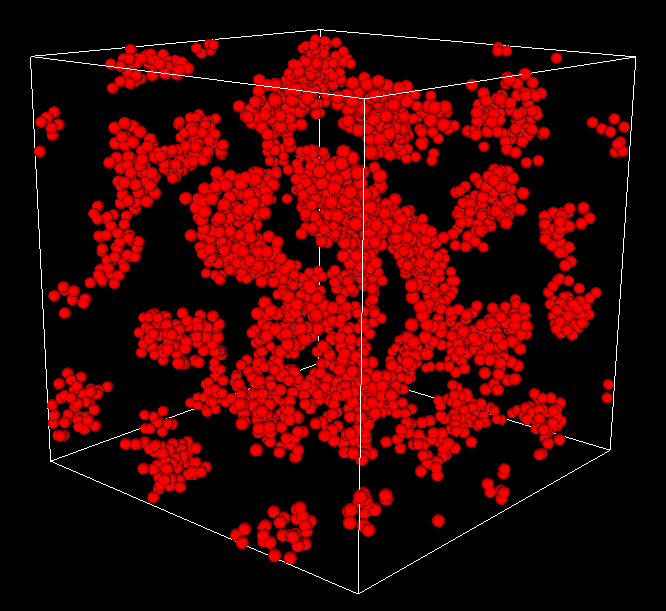
\includegraphics[width=45mm]{./fig/Snap.png}
	\label{fig: snap}
	\caption{Snapshot of the Model Network using A1B18A1 Triblock Polymer ($a_{AB} = 80$)}
	\end{center}
%\vspace{-3\baselineskip}
\end{wrapfigure}

粒子間相互作用は、保存力 $\mathbf{F}_{ij}^C$ に含まれる相互作用パラメータ $a_{ij}$ によって、以下のように表される。
\begin{equation}
\mathbf{F}_{ij}^C =
        	a_{ij} w^C (|\mathbf{r}_{ij}|) \dfrac{\mathbf{r}_{ij}}{|\mathbf{r}_{ij}|} \quad (|\mathbf{r}_{ij}| < r_c)
\end{equation}
なお、$\mathbf{r}_{ij} (=\mathbf{r}_i - \mathbf{r}_j)$ は粒子間距離、$w^C (|\mathbf{r}_{ij}|)$ は粒子間距離に応じた重み関数であり、 r$_c$ はカットオフ距離を表す。

密度 $\rho =3$ の場合は、一般に、同種ビーズ間の $a_{ii}$ は 25 と設定される。
異種粒子間の斥力は、この $a_{ij}$ の増分 $\Delta a$ で表現でき、フローリー・ハギンス格子モデルにおける $\chi$ パラメタと \eqref{eq:achi} 式に示したように相関が取れることが報告されている~\cite{Groot1997}。
\begin{equation}
\dfrac{\chi N k_B T}{\Delta a} = (0.306 \pm 0.003) N
\label{eq:achi}
\end{equation}



今回、テレケリックポリマーの計算モデルとして、20 個のビーズから成る A1B18A1 トリブロックポリマーを採用した。
%使用し、トリブロックポリマーの末端が作るクラスターからの引き抜きを観察した。
計算条件は、密度 $\rho =3$ とし、A1B18A1 トリブロックポリマー 1200 本、総ビーズ数は 24,000個とした。
A, B ビーズ間に斥力を設定($a_{AB} = 25, 40, 50, 60, 70, 80$)し、シミュレーションを行った。
これは、ジブロックポリマーとして考えた場合に、$\chi N \simeq 0 \sim 170$ 程度に対応すると考えることができる。


\begin{wrapfigure}{r}{50mm}
\vspace{-1\baselineskip}
	\begin{center}
	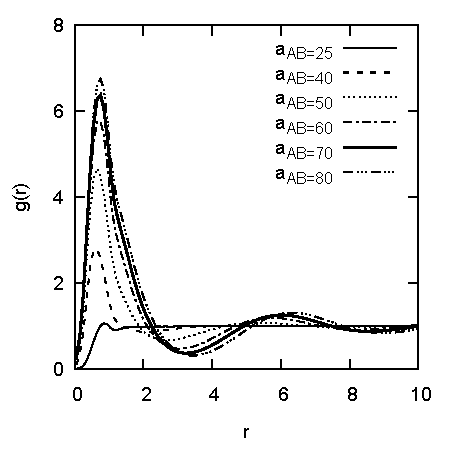
\includegraphics[width=50mm]{./fig/gr_all_mono.pdf}
	\vspace{-1\baselineskip}
	\label{fig: gr}
	\caption{g(r) for A beads with various  $a_{AB}$}
	\end{center}
\vspace{-1\baselineskip}
\end{wrapfigure}

任意の時間の構造緩和計算の後、応力の自己相関から応力緩和関数 $G(t)$ を求め、長時間領域での終端緩和から流動に至る緩和時間を見積った。
一方、ミクロな構造からの緩和時間として、ポリマー鎖の末端間ベクトルの自己相関から緩和時間を算出した。
さらに、末端の A ビーズが偏析したドメインを解析し~\cite{Aoyagi2002, Arai2007}、ブリッジ比およびドメインからの引き抜きによる緩和時間を見積もった。


\section{結果と考察}

Fig.1 のポリマー末端の A ビーズだけを表示したスナップショット ($a_{AB} = 80$) より、末端の A ビーズが偏析したドメインを形成していることが確認できる。

\begin{wrapfigure}{r}{50mm}
\vspace{-0.5\baselineskip}
	\begin{center}
	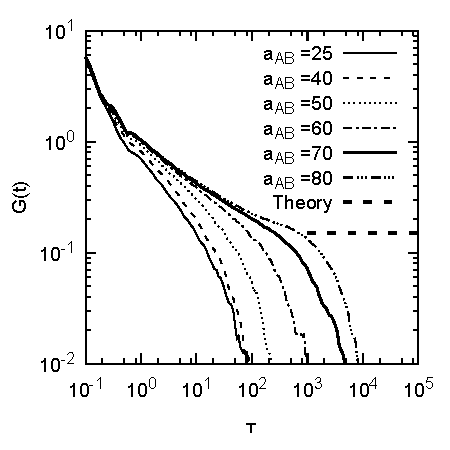
\includegraphics[width=50mm]{./fig/gt_all_mono.pdf}
	\vspace{-1\baselineskip}
	\label{fig: gt}
	\caption{G(t) calculated from autocorrelation of stress with various  $a_{AB}$}
	\end{center}
\vspace{-1\baselineskip}
\end{wrapfigure}


種々の $a_{AB}$ における A ビーズの動径分布関数 $g(r)$ を、Fig.2 に示した。
相互作用パラメタの増加に伴い、ドメイン内の A ビーズの偏析が増大し、さらに、長距離にわたる構造が形成されることが分かる。

応力緩和関数においては、相互作用パラメタ $a_{AB}$ の増加に伴い長時間領域でも応力が維持されるようになっていた(Fig.3)。
図中の点線は、古典ゴム弾性理論に基づき $G=\nu k_B T$ より算出したゴム状平坦部の弾性率であり、相互作用の増加により長時間領域の弾性率は平坦部へと漸近していた。

Tab.1 に、応力およびポリマー鎖の緩和時間を、可視化により得た引き抜きの緩和時間、ブリッジ比およびドメイン数とともに示した。
マクロな特性を反映する $\tau_{gt}$ は、ポリマー鎖全体の緩和を表す $\tau_{e2e}$ よりも小さく、引き抜きによる緩和時間の $\tau_{rels}$ と比較的よい相関を示し、末端の拘束解放により応力が緩和する機構が確認できた。



\begin{table}[h]
\centering
\caption{Relaxation Times ($\tau_{e2e}$, $\tau_{gt}$, $\tau_{rels}$), Bridge Ratio and Number of Domains}
\begin{tabular}{p{4em} p{4em} p{4em} p{4em} p{8em} p{10em}} \hline
\hfil $a_{AB}$ \hfil	&	\hfil $\tau_{e2e}$ \hfil	&	\hfil $\tau_{gt}$ \hfil	&	\hfil $\tau_{rels}$ \hfil	&	\hfil Bridge Ratio \hfil	&	\hfil Num. of Domains \hfil	\\ \hline \hline
\hfil 50 \hfil			&	\hfil 170 \hfil				&	\hfil 63 \hfil			&	\hfil 41 \hfil				&	\hfil 0.78 \hfil			&	\hfil 100 \hfil	\\ 
\hfil 60 \hfil			&	\hfil 650 \hfil				&	\hfil 250 \hfil			&	\hfil 160 \hfil				&	\hfil 0.77 \hfil			&	\hfil 60 \hfil	\\ 
\hfil 70 \hfil			&	\hfil 2200 \hfil			&	\hfil 910 \hfil			&	\hfil 990 \hfil				&	\hfil 0.73 \hfil			&	\hfil 46 \hfil	\\ 
\hfil 80 \hfil			&	\hfil 8200 \hfil			&	\hfil 2500 \hfil		&	\hfil 2600 \hfil			&	\hfil 0.74 \hfil			&	\hfil 40 \hfil	\\ \hline
\end{tabular}
\label{tbl:t}
\end{table}

%\begin{wraptable}{r}{80mm}
%\vspace{-1\baselineskip}
%\centering
%\caption{$\tau_{e2e}$, $\tau_{gt}$, $\tau_{rels}$ and Bridge Ratio with various $a_{AB}$}
%\vspace{5mm}
% \begin{tabular}{|p{2em}|p{3em}|p{3em}|p{3em}|p{4em}|} \hline
%\hfil $a_{AB}$ \hfil	&	\hfil $\tau_{e2e}$ \hfil	&	\hfil $\tau_{gt}$ \hfil	&	\hfil $\tau_{rels}$ \hfil	&	\hfil {\scriptsize Bridge Ratio} \hfil	\\ \hline \hline
%%\hfil 25 \hfil 		&	\hfil 48 \hfil				&	\hfil 25 \hfil			\\ \hline
%%\hfil 40 \hfil			&	\hfil 68 \hfil				&	\hfil 30 \hfil			\\ \hline
%\hfil 50 \hfil			&	\hfil 170 \hfil				&	\hfil 63 \hfil			&	\hfil 170 \hfil				&	\hfil 63 \hfil			\\ \hline
%%\hfil 60 \hfil			&	\hfil 650 \hfil				&	\hfil 250 \hfil			\\ \hline
%%\hfil 70 \hfil			&	\hfil 2200 \hfil			&	\hfil 910 \hfil			\\ \hline
%%\hfil 80 \hfil			&	\hfil 8200 \hfil			&	\hfil 2500 \hfil		\\ \hline
%\end{tabular}
% \label{tbl:t}
%\vspace{-1\baselineskip}
%\end{wraptable}

\section{おわりに}

DPD 法を用いた粗視化シミュレーションによりトリブロックポリマーの動的なネットワークの偏析度合いの可視化、および、緩和挙動の検討を行い、
マクロなパラメタである応力の緩和時間と、ミクロな構造である末端ビーズのドメインからの引き抜きから導出した緩和時間がよく相関することが分かった。

発表では、可視化の手法の詳細についても議論を行う予定である。

\bibliographystyle{achemso}
%{elsart-num}
%{junsrt-2}
\bibliography{C:/Dropbox/Tex/TeXworks/library.bib}

\end{document}